\section{拟Newton法}
\label{sec:mfo-quasi-newton}

Hessian难以形成或求解时，第~\ref{chap:quasi-newton}章用相邻两点的梯度差逐步学习曲率。流形上的困难在于，步、梯度差和曲率近似分属不同的切空间。这就需要回答：怎样把这些量放到同一切空间中，使割线关系和正定性仍然成立？

\subsection{黎曼BFGS}
\label{sec:mfo-rbfgs}

\paragraph{主要思想}
割线关系需要一个步和一个梯度差。把它们都放到新点$\bm{x}^{+}=R_{\bm{x}}(\alpha\bm{d})$的切空间：
\begin{equation}
 \bm{s}=\mathcal{T}_{\bm{x}\to\bm{x}^{+}}(\alpha\bm{d}),\qquad
 \bm{y}=\bm{g}^{+}-\mathcal{T}_{\bm{x}\to\bm{x}^{+}}(\bm{g}).
 \label{eq:mfo-curvature-pair}
\end{equation}
这样$\bm{s},\bm{y}\in T_{\bm{x}^{+}}M$，内积用该点的度量计算。

旧的近似算子$\bm{B}$作用在$T_{\bm{x}}M$上，也要搬过去。自然的办法如图~\ref{fig:mfo-operator-square}所示，先搬回旧切空间，作用$\bm{B}$，再搬到新切空间：
\begin{equation}
 \widetilde{\bm{B}}=\mathcal{T}\,\bm{B}\,\mathcal{T}^{-1}.
 \label{eq:mfo-operator-transport}
\end{equation}

\begin{BookInlineFigure}
 \centering
 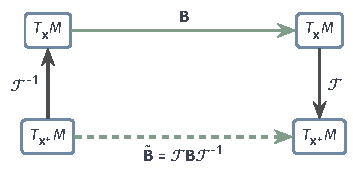
\includegraphics[width=59.8mm]{figures/05-optimization/06-constrained-optimization/tikz/mfo-operator-square/figure.pdf}
 \caption{曲率算子的搬运。绿色实线是旧切空间上的算子，虚线是新切空间上的算子，它由另外三段复合而成：先用$\mathcal{T}^{-1}$回到旧切空间，作用$\bm{B}$，再用$\mathcal{T}$搬到新切空间。}
 \label{fig:mfo-operator-square}
\end{BookInlineFigure}

这个构造对$\mathcal{T}$有要求。若$\mathcal{T}$等距，则$\widetilde{\bm{B}}$仍是自伴的，正定性也保留，因为
\[
 \langle\bm{u},\widetilde{\bm{B}}\bm{u}\rangle=\langle\mathcal{T}^{-1}\bm{u},\bm{B}\mathcal{T}^{-1}\bm{u}\rangle.
\]

等距这一条不能省略。在标准正交坐标下取$\mathcal{T}=\operatorname{diag}(1,\tfrac12)$，这是一个把第二个方向缩短的非等距映射。取对称正定的$\bm{B}$，计算得到
\[
 \bm{B}=\begin{bmatrix}2&1\\1&2\end{bmatrix},\qquad
 \mathcal{T}\bm{B}\mathcal{T}^{-1}=\begin{bmatrix}2&2\\\tfrac12&2\end{bmatrix},
\]
这个矩阵已经不对称了。所以投影搬运不能照搬式~\eqref{eq:mfo-operator-transport}，通常要改用等距搬运，或在搬运后作自伴化处理。

在$T_{\bm{x}^{+}}M$上做欧氏BFGS公式的类比，\term{黎曼BFGS}（Riemannian BFGS）的更新是
\begin{equation}
 \bm{B}^{+}[\bm{u}]=\widetilde{\bm{B}}[\bm{u}]-\frac{\langle\widetilde{\bm{B}}\bm{s},\bm{u}\rangle}{\langle\bm{s},\widetilde{\bm{B}}\bm{s}\rangle}\widetilde{\bm{B}}\bm{s}+\frac{\langle\bm{y},\bm{u}\rangle}{\langle\bm{y},\bm{s}\rangle}\bm{y}.
 \label{eq:mfo-rbfgs}
\end{equation}

代入$\bm{u}=\bm{s}$，前两项抵消，第三项给出$\bm{B}^{+}[\bm{s}]=\bm{y}$，这是新切空间内的割线关系。

记$\bm{W}$为$\bm{B}$的逆，$\rho=1/\langle\bm{s},\bm{y}\rangle$。在等距搬运下，用第~\ref{chap:quasi-newton}章的做法可得逆形式，它能直接给出方向$\bm{d}=-\bm{W}\bm{g}$，不必解方程：
\begin{equation}
 \bm{W}^{+}[\bm{u}]=\bm{V}^{*}\widetilde{\bm{W}}\bm{V}[\bm{u}]+\rho\langle\bm{s},\bm{u}\rangle\bm{s},\qquad
 \bm{V}[\bm{u}]=\bm{u}-\rho\langle\bm{s},\bm{u}\rangle\bm{y},
 \label{eq:mfo-rbfgs-inverse}
\end{equation}
其中$\bm{V}^{*}$是$\bm{V}$关于度量的伴随算子：
\[
 \bm{V}^{*}[\bm{u}]=\bm{u}-\rho\langle\bm{y},\bm{u}\rangle\bm{s}.
\]

\paragraph{曲率条件}
要使$\bm{B}^{+}$保持正定，需要$\langle\bm{s},\bm{y}\rangle>0$。欧氏情形由Wolfe条件保证，流形上要重新核对。设$\mathcal{T}$等距，由式~\eqref{eq:mfo-curvature-pair}，
\[
 \langle\bm{s},\bm{y}\rangle=\alpha\langle\mathcal{T}\bm{d},\bm{g}^{+}\rangle-\alpha\langle\bm{d},\bm{g}\rangle.
\]

Wolfe条件控制的量是沿回缩曲线的导数，记回缩曲线在新点的速度为$\mathcal{T}^{\mathrm{D}}\bm{d}$：
\[
 \langle\bm{g}^{+},\mathcal{T}^{\mathrm{D}}\bm{d}\rangle\geq c_2\langle\bm{g},\bm{d}\rangle.
\]
这和上一式的$\langle\mathcal{T}\bm{d},\bm{g}^{+}\rangle$是不同的量。两者若只差一个正因子$b$，即
\[
 \mathcal{T}\bm{d}=b\,\mathcal{T}^{\mathrm{D}}\bm{d},
\]
代入就有
\begin{equation}
 \langle\bm{s},\bm{y}\rangle\geq\alpha(bc_2-1)\langle\bm{g},\bm{d}\rangle.
 \label{eq:mfo-locking}
\end{equation}
下降方向满足$\langle\bm{g},\bm{d}\rangle<0$，所以$bc_2<1$时右端为正。

球面上用平行移动沿大圆走，方向恰好与回缩曲线同向。第~\ref{sec:mfo-transport}节的微分回缩长度是$\lVert\bm{d}\rVert_2/r^2$，平行移动保持长度，所以$b=r^2=1+\alpha^2\lVert\bm{d}\rVert_2^2$。贯穿例第$0$轮$\alpha=\tfrac12$，$b=\tfrac{98}{81}\approx1.21$，只要$c_2<0.826$就满足。

不满足上述配套关系时，曲率条件没有保证，要在运行中检查：若$\langle\bm{s},\bm{y}\rangle$不够大，就跳过这一次更新，只保留搬运后的$\widetilde{\bm{W}}$。

\needspace{6\baselineskip}
\paragraph{变量}
\begin{itemize}
 \item $\bm{x}^{(t)}$：当前点；$\bm{g}^{(t)}$：黎曼梯度，存它在切空间基下的二维坐标。
 \item $(\bm{E}_1^{(t)},\bm{E}_2^{(t)})$：切空间的标准正交基，用平行移动从上一轮搬来。
 \item $\bm{W}^{(t)}$：逆曲率近似，$2\times2$对称正定矩阵。
 \item $\bm{s},\bm{y}$：曲率对的二维坐标；$\rho=1/\langle\bm{s},\bm{y}\rangle$。
\end{itemize}

因为基是用平行移动搬过来的，向量的搬运在坐标上什么也不用做，式~\eqref{eq:mfo-operator-transport}也变成矩阵不变。这是采用等距搬运的计算便利。

\paragraph{初始化}
取$\bm{W}^{(0)}=\bm{I}_2$，基取$\bm{E}_1,\bm{E}_2$。例中起点是$\bm{x}^{(0)}=\tfrac13(2,2,1)^\top$，$\bm{g}^{(0)}$的坐标是$(\tfrac29,-\tfrac89)^\top$。

\needspace{6\baselineskip}
\paragraph{每轮更新}
\begin{enumerate}
 \item 算方向的坐标$\bm{d}^{(t)}=-\bm{W}^{(t)}\bm{g}^{(t)}$。例中第$0$轮是$(-\tfrac29,\tfrac89)^\top$，与梯度下降相同。

 \item 沿回缩线搜索得到$\alpha^{(t)}$，回缩得到$\bm{x}^{(t+1)}$。例中$\alpha=\tfrac12$，$\bm{x}^{(1)}$与第~\ref{sec:mfo-rgd}节相同。

 \item 用式~\eqref{eq:mfo-parallel-transport}搬运基，并算新梯度的坐标。例中
 \[
  \bm{g}^{(1)}\approx(-0.3938,\ -0.2433)^\top.
 \]

 \item 由式~\eqref{eq:mfo-curvature-pair}算曲率对。平行移动下坐标不变，例中
 \[
  \begin{gathered}
  \bm{s}=\frac12\bm{d}^{(0)}\approx(-0.1111,\ 0.4444)^\top,\\
  \bm{y}=\bm{g}^{(1)}-\bm{g}^{(0)}\approx(-0.6160,\ 0.6456)^\top.
  \end{gathered}
 \]

 \item 检查曲率。例中$\langle\bm{s},\bm{y}\rangle\approx0.3554>0$，可以更新，$\rho\approx2.8139$。

 \item 由式~\eqref{eq:mfo-rbfgs-inverse}更新$\bm{W}$。例中
 \[
  \bm{W}^{(1)}\approx\begin{bmatrix}0.7274&0.5219\\0.5219&1.1864\end{bmatrix}.
 \]
\end{enumerate}

第$1$轮方向的坐标是
\[
 \bm{d}^{(1)}=-\bm{W}^{(1)}\bm{g}^{(1)}\approx(0.4134,\ 0.4941)^\top,
\]
方向导数约为$-0.2830$，下降。试探$\alpha=1$得到
\[
 \bm{x}^{(2)}\approx(0.9955,-0.0010,-0.0944)^\top,\qquad f\approx0.5134,\qquad\lVert\bm{g}^{(2)}\rVert_2\approx0.2819.
\]

下面对照$\bm{x}^{(1)}$处真实的黎曼Hessian与$\bm{B}^{(1)}=(\bm{W}^{(1)})^{-1}$的坐标：
\[
 \bm{H}^{(1)}\approx\begin{bmatrix}1.47&-1.14\\-1.14&1.65\end{bmatrix},\qquad
 \bm{B}^{(1)}\approx\begin{bmatrix}2.01&-0.88\\-0.88&1.23\end{bmatrix}.
\]

只做一次更新，曲率对只在$\bm{s}$方向上提供信息，整个矩阵还不准确，割线方向上$\bm{B}^{(1)}\bm{s}=\bm{y}$精确成立。当$\lVert\bm{g}^{(t)}\rVert_2\leq10^{-6}$时结束，最终得到$\bm{x}^{(T)}\approx\pm\bm{e}_1$。

\paragraph{保证的来源}
下降性来自$\bm{W}$的正定性，而正定性要有三个条件同时成立：正定初值、保持自伴性和内积的搬运、每轮$\langle\bm{s},\bm{y}\rangle>0$。线搜索和回缩若不满足前述配套，后者就必须靠运行中检查来维持。

局部超线性收敛的结论针对具体的算法版本。已有的分析通常假定等距搬运、Wolfe型线搜索，以及类似式~\eqref{eq:mfo-locking}的配套条件；证明需要处理搬运带来的额外误差项，篇幅较长，读者可查阅黎曼拟Newton方法的专门文献。使用投影搬运、Armijo线搜索的简化版本在实际中也常常有效，但这些保证不能直接移用。

\subsection{有限记忆方法}
\label{sec:mfo-lbfgs}

\paragraph{主要思想}
稠密的$\bm{W}$要占$O(n^2)$存储，且每轮都要搬运一个算子。第~\ref{chap:quasi-newton}章的L-BFGS只保留最近$m$对$(\bm{s},\bm{y})$，用两层递推算出$\bm{W}\bm{g}$，流形上的版本思路相同，只是这些向量要跟着当前点走。

每次迭代后，把所存的向量对都搬到新切空间。递推仍是第~\ref{chap:quasi-newton}章的式子，内积换成当前点的度量。第一层从最新一对到最旧一对，初始$\bm{q}=\bm{g}$：
\begin{equation}
 \xi_j=\rho_j\langle\bm{s}_j,\bm{q}\rangle,\qquad
 \bm{q}\leftarrow\bm{q}-\xi_j\bm{y}_j.
 \label{eq:mfo-lbfgs-loop1}
\end{equation}

中间取$\bm{z}=\gamma\bm{q}$，尺度用最新的一对计算：
\[
 \gamma=\frac{\langle\bm{s},\bm{y}\rangle}{\langle\bm{y},\bm{y}\rangle}.
\]

第二层从最旧一对到最新一对：
\begin{equation}
 \eta_j=\rho_j\langle\bm{y}_j,\bm{z}\rangle,\qquad
 \bm{z}\leftarrow\bm{z}+(\xi_j-\eta_j)\bm{s}_j.
 \label{eq:mfo-lbfgs-loop2}
\end{equation}
最后的搜索方向是$\bm{d}=-\bm{z}$。

用$m=1$在贯穿例的第$1$轮算一遍，曲率对取上一小节的结果。第一层给出
\[
 \xi\approx-0.1811,\qquad\bm{q}\approx(-0.5053,\ -0.1263)^\top.
\]

中间$\gamma\approx0.4463$，所以$\bm{z}\approx(-0.2255,-0.0564)^\top$。第二层$\eta\approx0.2885$，于是
\[
 \bm{z}\approx(-0.1734,\ -0.2651)^\top,\qquad\bm{d}\approx(0.1734,\ 0.2651)^\top.
\]
方向导数约为$-0.1328$，是下降方向。它与完整BFGS的$(0.4134,0.4941)^\top$方向相近、长度不同，因为初始尺度从$\bm{I}$换成了$\gamma\bm{I}$。

\paragraph{历史长度与成本}
增大$m$减少迭代数，但每轮要搬运和内积的向量也增多。图~\ref{fig:mfo-lbfgs-memory}是$n=500$的实验，$m$从$1$增加到$50$，迭代数从$268$降到$141$，降幅不到一半，而按每轮$(3+10m)$次向量运算的粗略模型，总运算量却增加了约$20$倍。

\begin{BookInlineFigure}
 \centering
 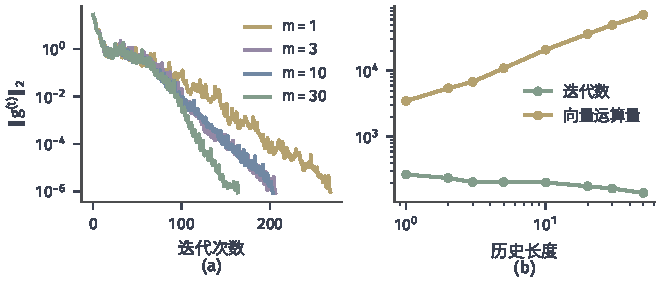
\includegraphics[width=112.0mm]{figures/05-optimization/06-constrained-optimization/matplotlib/mfo-lbfgs-memory/figure.pdf}
 \caption{$n=500$，$\bm{A}$的特征值在$1$到$100$之间等距，随机起点固定，使用平行移动的有限记忆黎曼BFGS，容差$\lVert\bm{g}\rVert_2\leq10^{-6}$。(a)~不同历史长度$m$的梯度范数。(b)~达到容差的迭代数（绿）和按每轮$3+10m$次向量运算估算的总运算量（黄）。}
 \label{fig:mfo-lbfgs-memory}
\end{BookInlineFigure}

这个实验中$\bm{A}$是对角阵，乘一次很便宜，搬运的代价显得突出。若$\bm{A}$乘向量很昂贵，或回缩的代价高，向量运算占比就小，较大的$m$更合算。

历史信息被截断后，完整BFGS的局部结论不再自动成立。有限记忆方法的曲率近似只包含$m$个方向，一般只有线性收敛的保证，这与欧氏情形一致。此外，为降低成本，一些实现只在需要时才搬运向量，这也属于另一种算法版本，其性质要另行核对。
